% !TeX root = ../main.tex

% Edit this title for each week's entry.
\section{Week 2 - Cash-flow Analysis}

\newlecture[Cash-flow Diagrams]

\begin{definition}[Cash-flow Diagram]
    A simple graph summarizing the \textbf{timing} and \textbf{magnitude} of
    cash-flows. The $x$-axis is discrete time periods; the (implicit)
    $y$-axis is the size and direction of each cash-flow, drawn as a
    vertical arrow: an \textbf{up} arrow is a receipt (inflow, $+\$$), a
    \textbf{down} arrow is a disbursement (outflow, $-\$$).
\end{definition}

\begin{center}
    \begin{tikzpicture}[scale=0.9]
        \draw[->] (0,0) -- (5,0) node[right] {\scriptsize time};
        \foreach \x in {0,1,2,3,4}{\fill (\x,0) circle (1.2pt);}
        \draw[->,thick,green!50!black] (1,0) -- (1,1) node[above] {\scriptsize $+\$$};
        \draw[->,thick,red!70!black] (3,0) -- (3,-1) node[below] {\scriptsize $-\$\$$};
    \end{tikzpicture}
    \\[2pt] \textit{\small Up = inflow (receipt); down = outflow (disbursement)}
\end{center}

\begin{definition}[Cash-flow Table]
    A table showing the money consequences of a situation and the timing
    of the cash-flows: for each point in time, the activity and the
    resulting cash-flow. Costs/benefits occurring at the start, during, or
    end of a project are together called the \textbf{project life-cycle
    costs}.
\end{definition}

\begin{remark}[Project Life-Cycle Cost Categories]
    \begin{itemize}
        \item \textbf{Start}: \textbf{First (capital) cost} --- expense to
        build/buy and install.
        \item \textbf{During}: \textbf{Revenues (sales)} --- receipts from
        sale of products/services; \textbf{O\&M costs} --- expenses
        incurred on a regular basis (electricity, labour, repairs);
        \textbf{Overhaul} --- a major capital expenditure partway through
        the asset's life.
        \item \textbf{End}: \textbf{Salvage value} --- net receipt from
        sale/disposal at the end of the asset's \emph{useful} life;
        \textbf{Scrap value} --- value of the materials at the end of the
        asset's \emph{physical} life; \textbf{Disposal costs} --- cost to
        dispose of waste (removal, shipping, tipping fees, etc.).
    \end{itemize}
\end{remark}

\begin{remark}[Diagram Conventions]
    \begin{itemize}
        \item Time $0$ is the start of period 1; the end of period $N$ is
        the start of period $N+1$.
        \item Unless stated otherwise: interest compounds once per
        period, and cash-flows occur at the \textbf{end} of the period.
        \item Cash-flows occurring \emph{during} a period are summed and
        accounted for at the \textbf{end} of that period.
    \end{itemize}
\end{remark}

\begin{example}[Loan Repayment Diagram]
    \$1,000 is borrowed on January 1 and repaid in 6 monthly installments
    of \$172.50 ($i=1\%$ per month). From the \textbf{borrower's}
    perspective: an inflow of \$1,000 at $t=0$, and outflows of \$172.50
    at $t=1,\dots,6$. From the \textbf{bank's} perspective the diagram
    flips: an outflow of \$1,000 at $t=0$, and inflows of \$172.50 at
    $t=1,\dots,6$.
\end{example}

\begin{center}
    \begin{minipage}{0.46\linewidth}\centering
        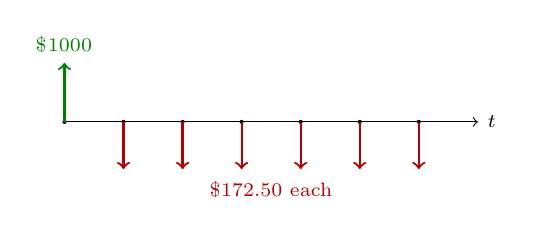
\begin{tikzpicture}[scale=0.75]
            \draw[->] (0,0) -- (7,0) node[right] {\scriptsize $t$};
            \foreach \x in {0,...,6}{\fill (\x,0) circle (1pt);}
            \draw[->,thick,green!50!black] (0,0) -- (0,1) node[above] {\scriptsize \$1000};
            \foreach \x in {1,...,6}{\draw[->,thick,red!70!black] (\x,0) -- (\x,-0.8);}
            \node[red!70!black] at (3.5,-1.15) {\scriptsize \$172.50 each};
        \end{tikzpicture}
        \\[2pt] \textit{\small Borrower}
    \end{minipage}
    \hfill
    \begin{minipage}{0.46\linewidth}\centering
        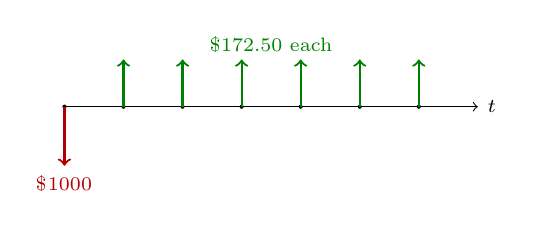
\begin{tikzpicture}[scale=0.75]
            \draw[->] (0,0) -- (7,0) node[right] {\scriptsize $t$};
            \foreach \x in {0,...,6}{\fill (\x,0) circle (1pt);}
            \draw[->,thick,red!70!black] (0,0) -- (0,-1) node[below] {\scriptsize \$1000};
            \foreach \x in {1,...,6}{\draw[->,thick,green!50!black] (\x,0) -- (\x,0.8);}
            \node[green!50!black] at (3.5,1.05) {\scriptsize \$172.50 each};
        \end{tikzpicture}
        \\[2pt] \textit{\small Bank (flipped)}
    \end{minipage}
\end{center}

\newlecture[Categories of Regular Cash-flows]

\begin{definition}[Single Payment/Receipt]
    A single cash-flow $P$ (now) or $F$ (in the future), occurring only
    once, $N$ periods apart.
\end{definition}

\begin{center}
    \begin{tikzpicture}[scale=0.8]
        \draw[->] (0,0) -- (4,0) node[right] {\scriptsize $t$};
        \fill (0,0) circle (1pt); \fill (3,0) circle (1pt);
        \node at (0,-0.35) {\scriptsize $0$};
        \node at (3,-0.35) {\scriptsize $N$};
        \draw[->,thick] (0,0) -- (0,-0.9) node[below] {\scriptsize $P$};
        \draw[->,thick] (3,0) -- (3,0.9) node[above] {\scriptsize $F$};
    \end{tikzpicture}
\end{center}

\begin{definition}[Perpetuity]
    A constant cash-flow $A$ occurring every period, forever (an
    \emph{infinite annuity}).
\end{definition}

\begin{center}
    \begin{tikzpicture}[scale=0.8]
        \draw[->] (0,0) -- (5.5,0) node[right] {\scriptsize $t$};
        \foreach \x in {1,...,5}{\fill (\x,0) circle (1pt); \draw[->,thick] (\x,0) -- (\x,0.8);}
        \node at (1,1.05) {\scriptsize $A$};
        \node at (5.8,0.4) {\scriptsize $\cdots$};
    \end{tikzpicture}
\end{center}

\begin{definition}[Annuity]
    A constant cash-flow $A$ occurring every period, for a \emph{finite}
    number of periods $N$.
\end{definition}

\begin{center}
    \begin{tikzpicture}[scale=0.8]
        \draw[->] (0,0) -- (5,0) node[right] {\scriptsize $t$};
        \foreach \x in {1,...,4}{\fill (\x,0) circle (1pt); \draw[->,thick] (\x,0) -- (\x,0.8);}
        \node at (1,1.05) {\scriptsize $A$};
        \node at (4,-0.35) {\scriptsize $N$};
    \end{tikzpicture}
\end{center}

\begin{definition}[Arithmetic Gradient]
    A cash-flow that grows (or shrinks) by the same \emph{amount} $G$
    each period, starting from a base $A'$ at $t=1$:
    \[A',\ A'+G,\ A'+2G,\ \dots,\ A'+(N-1)G.\]
\end{definition}

\begin{center}
    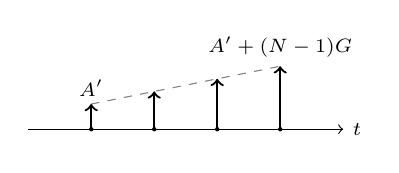
\begin{tikzpicture}[scale=0.8]
        \draw[->] (0,0) -- (5,0) node[right] {\scriptsize $t$};
        \draw[dashed,gray] (1,0.4) -- (4,1.0);
        \foreach \x/\h in {1/0.4,2/0.6,3/0.8,4/1.0}{\fill (\x,0) circle (1pt); \draw[->,thick] (\x,0) -- (\x,\h);}
        \node at (1,0.65) {\scriptsize $A'$};
        \node at (4,1.3) {\scriptsize $A'+(N-1)G$};
    \end{tikzpicture}
    \\[2pt] \textit{\small Arrow tops grow \emph{linearly} (straight trend line)}
\end{center}

\begin{definition}[Geometric Gradient]
    A cash-flow that grows (or shrinks) by the same \emph{percentage} $g$
    each period, starting from $A$ at $t=1$:
    \[A,\ A(1+g),\ A(1+g)^2,\ \dots,\ A(1+g)^{N-1}.\]
\end{definition}

\begin{center}
    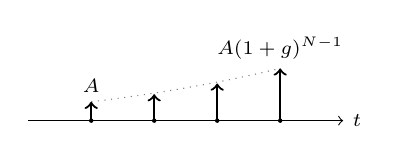
\begin{tikzpicture}[scale=0.8]
        \draw[->] (0,0) -- (5,0) node[right] {\scriptsize $t$};
        \draw[dotted,gray] (1,0.3) .. controls (2,0.42) and (3,0.59) .. (4,0.83);
        \foreach \x/\h in {1/0.3,2/0.42,3/0.59,4/0.83}{\fill (\x,0) circle (1pt); \draw[->,thick] (\x,0) -- (\x,\h);}
        \node at (1,0.55) {\scriptsize $A$};
        \node at (4,1.15) {\scriptsize $A(1+g)^{N-1}$};
    \end{tikzpicture}
    \\[2pt] \textit{\small Arrow tops grow \emph{exponentially} (curved trend line)}
\end{center}

\newlecture[Cash-flow Equivalence]

\begin{definition}[Mathematical Equivalence]
    A consequence of the mathematical relationship between time and
    money. Two cash-flows $P_t$ (at time $t$) and $F_{t+N}$ (at time
    $t+N$) are equivalent at rate $i$ if
    \[F_{t+N} = P_t(1+i)^N \iff P_t = \frac{F_{t+N}}{(1+i)^N}.\]
    If a further cash-flow $F_{t+N+M}$ is also equivalent to $P_t$, then
    $F_{t+N+M} = F_{t+N}(1+i)^M$: equivalent amounts compound/discount
    consistently with each other.
\end{definition}

\begin{center}
    \begin{tikzpicture}[scale=0.8]
        \draw[->] (0,0) -- (5,0) node[right] {\scriptsize $t$};
        \fill (0,0) circle (1.2pt); \fill (3,0) circle (1.2pt);
        \node at (0,-0.35) {\scriptsize $t$};
        \node at (3,-0.35) {\scriptsize $t+N$};
        \draw[->,thick] (0,0) -- (0,-0.9) node[below] {\scriptsize $P_t$};
        \draw[->,thick] (3,0) -- (3,0.9) node[above] {\scriptsize $F_{t+N}$};
        \node at (1.5,0.55) {\scriptsize $\equiv$};
    \end{tikzpicture}
\end{center}

\begin{definition}[Market Equivalence]
    A consequence of being able to exchange one cash-flow for another at
    \emph{zero cost}. Exchanging a future cash-flow for a present one is
    \textbf{borrowing}; giving up a present cash-flow for a future one is
    \textbf{lending/investing}. In real markets, borrowing and lending
    rates usually differ.
\end{definition}

\begin{example}[T-bill Market Equivalence]
    A \$1,000 T-bill maturing in 6 months currently sells for \$990.10.
    The market has agreed this corresponds to an interest rate of 1\%
    over 6 months.
\end{example}

\begin{definition}[Decisional Equivalence]
    Two cash-flows $P_t$ and $F_{t+N}$ are equivalent for a decision
    maker if they are \emph{indifferent} between them. Here the interest
    rate is not known a priori --- instead, an \emph{implied} rate can be
    backed out from the decision that the two are equivalent.
\end{definition}

\begin{example}[Implied Interest Rate]
    A manufacturer needs 1,000~kg of aluminium on August 15 but is
    offered 1,100~kg on August 22 instead (same price, paid at the end
    of August). Accepting the delay implies an interest rate of 10\% for
    one week.
\end{example}

\begin{remark}
    Financial analysis uses \textbf{mathematical} and \textbf{market}
    equivalence to decide whether to invest.
\end{remark}

\newlecture[Cash-flow Factors]

\begin{remark}[Standing Assumptions]
    Unless otherwise noted:
    \begin{enumerate}
        \item Interest compounds once per period.
        \item Cash-flow occurs at the end of the period.
        \item Time 0 is period 0, i.e.\ the start of period 1.
        \item All periods are the same length.
    \end{enumerate}
\end{remark}

\begin{definition}[Cash-flow Symbols]
    $P$: a single cash-flow today. $F$: a single cash-flow in the
    future. $A$: a finite series of equal cash-flows at regular
    intervals (annuity). $G$: a cash-flow growing by a fixed
    \emph{amount} each period (arithmetic gradient) or fixed
    \emph{percentage} $g$ each period (geometric gradient, ``Geom'').
\end{definition}

\begin{definition}[Factor Notation]
    $(X/Y,i,N)$ converts a cash-flow of type $Y$ into the equivalent
    amount of type $X$ at rate $i$ over $N$ periods: $X = Y\cdot
    (X/Y,i,N)$. E.g.\ $F = P(F/P,i,N)$; for geometric gradients,
    $P = G(P/\text{Geom},i,g,N)$.
\end{definition}

\begin{center}
    \begin{tabular}{ll}
        \toprule
        Factor & Name \\
        \midrule
        $(F/P,i,N)$ & Compound amount factor \\
        $(P/F,i,N)$ & Present worth factor \\
        $(A/F,i,N)$ & Sinking fund factor \\
        $(F/A,i,N)$ & Series compound amount factor \\
        $(A/P,i,N)$ & Capital recovery factor \\
        $(P/A,i,N)$ & Series present worth factor \\
        \bottomrule
    \end{tabular}
\end{center}

\begin{remark}[Relating Factors]
    Factors invert: since $P = A(P/A,i,N)$ and $A = P(A/P,i,N)$, we get
    $(A/P,i,N) = 1/(P/A,i,N)$. The same trick relates any pair of
    factors.
\end{remark}

\begin{definition}[Single-Payment Factors]
    \[(F/P,i,N) = (1+i)^N, \qquad (P/F,i,N) = (1+i)^{-N}.\]
\end{definition}

\begin{center}
    \begin{tikzpicture}[scale=1]
        \draw[->] (0,0) -- (4.6,0) node[right] {\scriptsize $N$};
        \draw[->] (0,0) -- (0,2.3) node[above] {\scriptsize $(P/F,i,N)$};
        \foreach \x/\lbl in {0/0,1/2,2/4,3/6,4/8}{
            \draw (\x,0.05) -- (\x,-0.05);
            \node[below] at (\x,-0.08) {\scriptsize \lbl};
        }
        \node[left] at (0,2) {\scriptsize $1.0$};
        \draw[thick,blue!60!black] plot coordinates
            {(0,2)(0.5,1.818)(1,1.652)(1.5,1.502)(2,1.366)(2.5,1.242)(3,1.128)(3.5,1.026)(4,0.934)};
    \end{tikzpicture}
    \\[2pt] \textit{\small $(1+i)^{-N}$ decays toward $0$ as $N$ grows (shown for $i=10\%$)}
\end{center}

\begin{example}[Present Value of a Perpetuity]
    A constant amount $A$ paid forever has finite present value:
    \[P = \frac{A}{1+i}+\frac{A}{(1+i)^2}+\cdots = \frac{A}{i}.\]
\end{example}

\begin{definition}[Present Worth of an Annuity]
    \[(P/A,i,N) = \frac{1}{i}-\frac{1}{i(1+i)^N}
    = \frac{(1+i)^N - 1}{i(1+i)^N}.\]
\end{definition}

\begin{definition}[Present Worth of an Arithmetic Gradient]
    For a gradient contributing $G,2G,\dots,(N-1)G$ starting at $t=2$
    (no cash-flow at $t=0$ or $t=1$):
    \[(P/G,i,N) = \frac{1}{i^2}\left(1-\frac{1+iN}{(1+i)^N}\right).\]
    A series with initial amount $A$ growing by $G$ each period splits
    into an annuity plus a gradient:
    \[P = A(P/A,i,N) + G(P/G,i,N).\]
\end{definition}

\begin{remark}[Sign Combinations for Arithmetic Gradients]
    Besides $G=0$, four cases: $A>0,\,G>0$ (positive, increasing);
    $A>0,\,G<0$ (positive, decreasing); $A<0,\,G>0$ (negative, becoming
    less so); $A<0,\,G<0$ (negative, becoming more so).
\end{remark}

\begin{definition}[Present Worth of a Geometric Gradient]
    For a series $A,\,A(1+g),\,A(1+g)^2,\dots$ starting at $t=1$:
    \[(P/\text{Geom},i,g,N) = \frac{1-\left(\frac{1+g}{1+i}\right)^N}{i-g}
    = \frac{(P/A,i_o,N)}{1+g}, \qquad i_o = \frac{1+i}{1+g}-1.\]
\end{definition}

\begin{remark}
    Regardless of the pattern, present value always follows from
    discounting each cash-flow individually and summing:
    \[\boxed{P = \sum_t \frac{F_t}{(1+i)^t}.}\]
\end{remark}

\newlecture[Worked Examples]

\begin{example}[Investment Decision]
    An investor can buy a tract of land that will be worth \$10,000 in
    six years. If the required rate of return is 8\%, the investor
    should be willing to pay $P = 10{,}000(P/F,8\%,6)$ now.
\end{example}

\begin{example}[Mortgage/Amortization]
    A \$300,000 mortgage at a nominal 9\% (compounded semi-annually) is
    amortized over 15 years. The monthly payment $A$ solves
    $300{,}000 = A(P/A,i_s,180)$, where $i_s$ is the effective monthly
    rate equivalent to the semi-annual nominal rate.
\end{example}

\begin{example}[Sinking Fund]
    A roof must be replaced in 10 years for an estimated \$28,000. The
    equal end-of-year deposits $A$ needed at 8\% interest solve
    $A = 28{,}000(A/F,8\%,10)$.
\end{example}

\begin{example}[Retirement Planning]
    Starting at age 20 and retiring at 65 (45 years), the equal
    end-of-year savings $A$ needed to reach \$1{,}000{,}000 at an average
    7\% return solve $A = 1{,}000{,}000(A/F,7\%,45)$; a higher rate
    (e.g.\ 10\%) reduces the required $A$.
\end{example}

\begin{example}[Uneven Annuity Segments]
    To fund withdrawals of \$2,000/year for 5 years followed by
    \$3,000/year for the next 3 years at 8\% interest, the deposit
    needed now is
    \[P = 2{,}000(P/A,8\%,5) + 3{,}000(P/A,8\%,3)(P/F,8\%,5),\]
    discounting the second annuity back to $t=5$ and then to $t=0$.
\end{example}

\begin{example}[Present Value with an Arithmetic Gradient]
    A machine costs \$155 to maintain this year, with maintenance
    costing \$35 more each subsequent year, over an 8-year life at 6\%
    interest. The present value of the maintenance cash-flow is
    \[P = 155(P/A,6\%,8) + 35(P/G,6\%,8).\]
    Adding an up-front overhaul cost simply adds that amount at $t=0$.
\end{example}

\begin{example}[Future Value with Periodic Dividends]
    \$100,000 is invested at 15\% (compounded annually, not paid out),
    with a \$5,000 dividend received every third year for 15 years and
    reinvested at the same 15\%. The total future value combines the
    compounded principal with the compounded value of each dividend.
\end{example}
